\documentclass{article}
\usepackage{polski}
\usepackage[utf8]{inputenc}
\usepackage{listings}
\usepackage{color}
\usepackage{verbatim}
\usepackage{hyperref}
\usepackage{graphics}
 \hypersetup{
    colorlinks=true,
    linkcolor=blue,
    filecolor=magenta,      
    urlcolor=cyan,
}
 
\urlstyle{same}
\definecolor{codegreen}{rgb}{0,0.6,0}
\definecolor{codepurple}{rgb}{0.58,0,0.82}
\definecolor{codegray}{rgb}{0.9,0.9,0.9}
 
\lstdefinestyle{mystyle}{
    backgroundcolor=\color{codegray},  
    commentstyle=\color{codegreen},
    keywordstyle=\color{blue},
    numberstyle=\tiny\color{black},
    stringstyle=\color{codepurple},
    basicstyle=\footnotesize,
    breaklines=true,                 
    captionpos=b,                    
    keepspaces=true,                 
    numbers=left,                    
    frame=single
}
 
\lstset{style=mystyle}

\title{Polecenia głosowe}
\author{Marcin Tomecki}
\date{June 2018}


\usepackage{graphicx}

\begin{document}
\begin{titlepage}
\centering
\Huge \textbf{RPG Utility Lite}\par
\Large \textbf{Dobry asystent każdego RPG-wicza}
\vfill
Wydział Matematyki Stosowanej\\Kierunek Informatyka semestr IV\par
\vfill
\vfill
\begin{flushright}
Piotr Samek\\
Marcin Tomecki\\
Tomasz Węcławski
\end{flushright}
Czerwiec 2018
\end{titlepage}
\tableofcontents
\newpage
\clearpage
\section{Historia zmian}
\textit{imię\_nazwisko | data | zmiana}\\
Marcin Tomecki                 | 06.06.2018              | Strona tytułowa\\
Wspólnie                       | 20.06.2018              | Prezentacja\\
Tomasz Węcławski               | 30.06.2018 - 01.07.2018 | Stworzenie bazy danych\\
Marcin Tomecki                 | 01.07.2018              | Podłączenie bazy danych pod Microsoft Azure\\
Piotr Samek i Tomasz Węcławski | 01.07.2018              | Testowanie połączenia i zapytań w bazie danych\\
Piotr Samek                    | 03.07.2018              | Dokumentacja BD\\
Tomasz Węcławski               | 04.07.2018              | Aktualizacja bazy danych
\newpage
\section{Wstęp}
\textbf{RPG Utility Lite} to aplikacja wspomagająca graczy tabletop RPG, która
obsługiwać będzie bazę danych z informacjami dotyczącymi świata gry, jak i pozwoli
stworzyć i przechowywać własne postacie.
\\Dzięki RPG Utility Lite możemy zamienić ogromną ilość makulatury w poręczne narzędzie, które będzie z nami zawsze i wszędzie.
\\Aplikacja pozwala również zaoszczędzić czas - zamiast wertować setki stron w poszukiwaniu pożądanej informacji, wystarczy wybrać w odpowiednią tematykę, parę kliknięć i gotowe!
\\\\Zakres projektu obejmuje:
\begin{itemize}
    \item stworzenie aplikacji
    \item dobór odpowiednich narzędzi
    \item wybór odpowiedniego schematu działania
    \item podział obowiązków
    \item wykonanie
\end{itemize}

\newpage
\section{Obsługa}
By móc korzystać z aplikacji potrzebne będzie własne konto użytkownika zabezpieczone hasłem.
\\Należy się zalogować, by po chwili móc się cieszyć dostępem do niezliczonej ilości informacji, co dotychczas było możliwe tylko dzięki posiadaniu ogromnej liczby, często nietanich, książek.
\\
\begin{figure}[h!]
\begin{center}
    
\centering
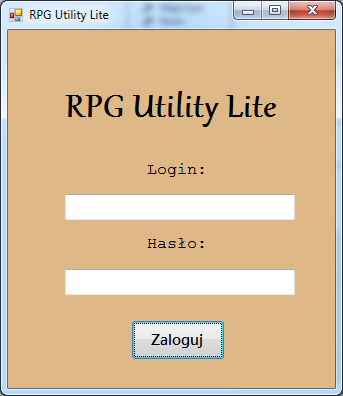
\includegraphics[]{ekranpowitalny.png}

\end{center}
\end{figure}
\newpage
Następnie wystarczy wybrać jeden spośród interesujących nas tematów:
\begin{figure}[h!]
\begin{center}
    
\centering
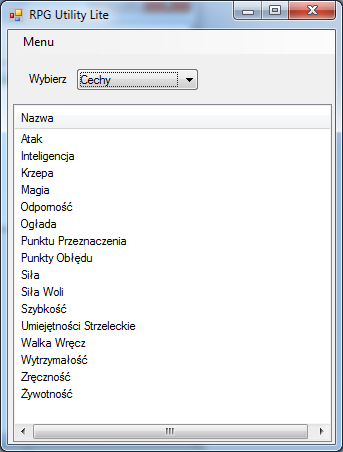
\includegraphics[]{cechy.png}

\end{center}
\end{figure}

\newpage
\section{Schemat projektu}
Utworzyliśmy relacyjną bazę danych, która jest zarządzana za pomocą
systemu \textit{Microsoft SQL Server 2017 (MS SQL)}. Podczas tworzenia aplikacji skorzystaliśmy z usługi \textit{Azure SQL Database}. Umożliwia ona zarządzanie bazą danych w chmurze, dzięki czemu można migrować bazy danych programu \textit{SQL Server} bez wprowadzania zmian w aplikacjach.
\subsection*{Diagram klas}
\begin{figure}[h!]
\begin{center}
    
\centering
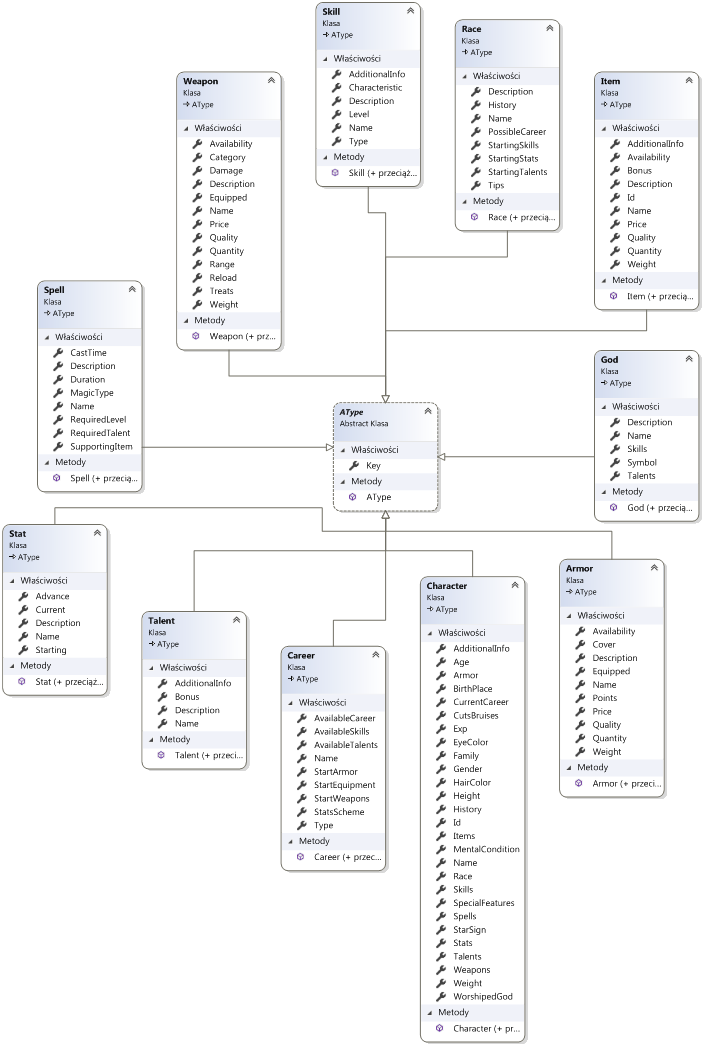
\includegraphics[height=400px]{Diagram_klas_UML.png}

\end{center}
\end{figure}

\newpage
\section{Szczegóły techniczne}
Po zaprojektowaniu modelu relacyjnego mogliśmy w miarę prosty sposób stworzyć bazę danych i dodać ją do projektu (solucji).
\\\\Przykładowa implementacja tabeli:
\begin{verbatim}
    CREATE TABLE [uni].[pos_bro] (
    [id_postaci]   INT       NOT NULL,
    [jakosc]       CHAR (30) NOT NULL,
    [bron]	    	   CHAR (50) NOT NULL FOREIGN KEY REFERENCES bronie(nazwa),
    [zaekwipowany] BIT       NULL,
    [ilosc]        INT       NULL,
    PRIMARY KEY CLUSTERED ([id_postaci] ASC, [jakosc] ASC, [bron] ASC),
    FOREIGN KEY ([id_postaci]) REFERENCES [n_uni].[postacie] ([id])
    );

\end{verbatim}

\newpage
\section{Problemy}
W trakcie tworzenia aplikacji napotkaliśmy (co zdarza się zawsze) kilka problemów:
\begin{itemize}
    \item Połączenie się z bazą \textit{Azure SQL Database} jako nowy uzytkownik może być problematyczne - trzeba dodać do bazy danego użytkownika poprzez podanie przez niego swojego adresu IP.
    \item Klucz główny w bazie nie może mieć typu \textit{ntext}.
    \\Rozwiązaniem problemu jest zamiana typu \textit{ntext} na \textit{nvarchar} z określoną ilością znaków, np. \textit{[nvarchar](20)}.
    \item Sam typ \textit{ntext} jest już przestarzały i zaleca się stosowanie \textit{[nvarchar](max)}.
    \item Bardzo ciężko jest napisać prosty skrypt obsługujący rejestrację.
    \\Samo dodanie użytkownika do bazy i dodanie go do listy użytkowników bazy w \textit{Azure SQL Database} wymaga bycia uprzednio połączonym i zalogowanym w bazie, mówiąc wprost - napisanie skryptu do rejestracji, nie sprzedając tym samym dostępu do całej bazy, jest bardzo trudne.
    \\Potencjalnym rozwiązaniem jest wysyłanie zapytania o dodanie do listy użytkowników przy rejestracji (przykładem jest oczekiwanie na akceptację dodania do danej grupy na \textit{Facebook'u}). Jest to jednak nieefektywne, gdyż chcielibyśmy mieć dostęp do informacji od razu po rejestracji - chyba, że mamy na tyle użyteczne informacje w przystępnej formie, że oczekiwanie jest tego warte.
    \item Przy zmianie tematu często wyrzucało błąd o niezamkniętym połączeniu.
    \\Wystarczyło wywołać prostą metodę
    \begin{verbatim}
        conn.Close();
    \end{verbatim}
    która zamyka obecne połączenie sql, dzięki czemu możemy wywołać nowe.
    \item Problemem jest też na pewno obszerność - wydawać się może, że jest to mała aplikacja, jednak ilość tematów, sekcji i informacji jest ogromna i w miarę rozbudowy, można się przez przypadek łatwo zgubić (i chodzi tutaj zdecydowanie o stronę programistyczną).
\end{itemize}

\section{Bibliografia}


\end{document}
